\chapter{Introduzione}
Che cosa sono l'analisi e la Progettazione
\begin{itemize}
    \item Analisi - Enfatizza un'investigazione di un problema e dei suoi
    requisiti, anzichè di una soluzione
    \item La progettazione enfatizza una soluzione concettuale che soddisfa i requisiti
    del problema
\end{itemize}
Fare la cosa giusta (analisi) e fare la cosa bene (progettazione)
\section{Analisi e Progettazione orientata agli oggetti}
L'analisi orientata agli oggetti enfatizza sull'identificazione dei concetti o
degli oggetti, nel dominio del problema.
\\ La progettazione orentata agli oggetti enfatizza sulla definizione di oggetti
software che collaborano per soddisfare i requisiti.
\paragraph*{Esempio} Oggetti - Aereo, Volo, Pilota ognuno con i propri attributi
(tipo basi di dati).
Analisi e progettazione hanno obiettivi diversi che venogno perseguiti in modi diversi,
sono comunque attività sinergiche.
\\ L'OO (Object Oriented) enfatizza la rappresentazione di oggetti
\paragraph*{Definizione dei casi d'uso}
I casi d'uso sono delle store scritte relative al mondo in cui il sistema
viene utilizzato.
\paragraph*{Definizione di un modello di dominio}
Un modello di dominio mostra i concetti o gli oggetti significativi del dominio,
con i relativi attributi e associazioni.
\begin{center}
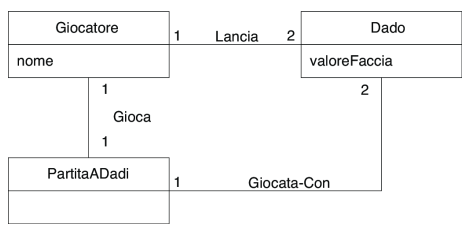
\includegraphics[width=100mm, scale=0.5]{modello_di_dominio_es.png}
\end{center}
\paragraph*{Definizione dei diagrammi di interazione}
Un diagramma di interazione mostra le collaborazioni tra oggetti software.
\begin{center}
    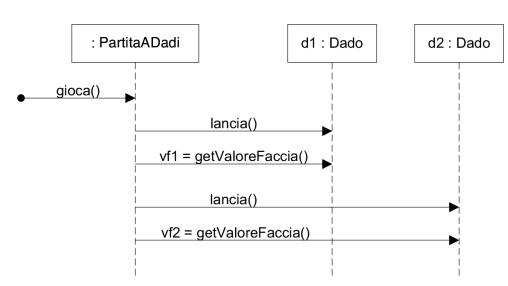
\includegraphics[width=100mm, scale=0.5]{diagramma_di_interazione_es.png}
\end{center}
\paragraph*{Definizioni dei diagramma delle classi di progetto}
Un diagramma delle classi di progetto mostra una vista statica delle definizioni
delle classi software, con i loro attributi e metodi.
\begin{center}
    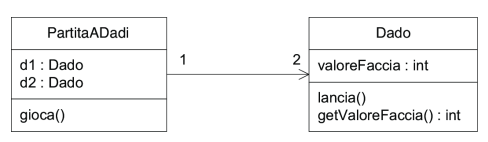
\includegraphics[width=100mm, scale=0.5]{diagramma_delle_classi_di_progetto.png}
\end{center}
Lo scopo di tutti questi diagrammi è facilitare la progettazione e il passaggio
da idea a codice.
\section{Che cosa è UML}
Unified Modelling Language (UML) è un linguaggio visuale di modellazione
dei sistemi e non solo.
Rappresenta una collezione di best practice di ingegneria, dimostratesi vincenti
nella modellazione di sistemi vasti e complessi. Dato che è lo standard de facto
favorisce la divulgazione di informazioni nella comunotà di ingegneri del software.
\\ \textbf{UML NON è una metodologia}
\begin{itemize}
    \item UML è un linguaggio visuale
    \item UP (Unified Process) è una metodologia
\end{itemize}
UML modella i sistemi come insiemi di oggetti che collaborano tra loro
\begin{itemize}
    \item Struttura Statica \begin{itemize}
        \item Quali tipo di oggetti sono necessari
        \item Come sono tra loro correlati
    \end{itemize}
    \item Struttura Dinamica \begin{itemize}
        \item Ciclo di vita di questi oggetti
        \item Come collaborano per fornire la funzionalità richieste
    \end{itemize}
\end{itemize}
\subsection{Tre modi per applicare UML}
\begin{itemize}
    \item UML come abbozzo
    \item UML come progetto
    \item UML come linguaggio di programmazione
\end{itemize}
\paragraph*{UML come Abbozzo} Diagrammi informali e incompleti (spesso abbozzati a mano)
che vengono creati per esplorare parti difficili dello spazio del problema o 
della soluzione, sfruttando l'espressività dei linguaggi visuali.
\paragraph*{UML come Progetto} Diagrammi di progetto relativamente dettagliati,
utilizzati per il reverse engineering, per la documentazione e per la comunicazione,
utilizzati quindi per visualizzare e comprendere meglio il codice esistente mediante
diagrammi UML.
\paragraph*{UML come linguaggio di programmazione} In questo caso il codice
viene generato direttamente e automaticamente da UML (approccio ancora in fase
di sviluppo).
\textbf{La modellazione agile enfatizza l'uso di UML come abbozzo}
\paragraph*{Due punti di vista per applicare UML}
\begin{itemize}
    \item Punto di vista concettuale - I diagrammi descrivono oggetti del mondo reale
    o in un dominio di interesse
    \item Punto di vista software - I diagrammi descrivono atrsazioni o componenti
    software
\end{itemize}
Entrambi usano la stessa notazione UML.
\subsection*{Il significato di classe nei diversi punti di vista}
Nell'UML grezzo, i rettangoli illustrati sono chiamati classi, questo termine
racchiude una varietà di casi: oggetti fisici, concetti astratti, elementi software, ecc.
\\ Il significato varia in base al diagramma di utilizzo, per fare chiarezza:
\begin{itemize}
    \item Classe concettuale - Oggetto o concetto del mondo reale - Significato
    attribuito nel \textbf{Modello di Dominio di UP}
    \item Classe software - Classe intesa come componente software (es. classe Java)
    - Significato attribuito nel \textbf{Modello di Progetto di UP}
\end{itemize}


